%
% $Id: ch03_thework.tex
%
%   *******************************************************************
%   * SEE THE MAIN FILE "AllegThesis.tex" FOR MORE INFORMATION.       *
%   *******************************************************************
%
\chapter{Method of Approach} \label{ch:method}
In this chapter, we discuss the implementation details for our system.  The
implementation can be broken into four distinct sections:

\begin{enumerate}
\item XML parsing
\item Intermediate representation
\item Simplified representation
\item Risk evaluation
\end{enumerate}

\section{XML Parsing} \label{sec:parse}

When CodeCover produces per-test coverage information, it stores the results in
a container.  Though CodeCover features several coverage report export types, 
including hierarchical HTML, these reports do not include all information
necessary for this project.  Specifically, these export formals only include
general per-test coverage information, displaying percent coverage for each test.
They do not include information related to precisely which tests executed each 
statement, which is a requirement for suspiciousness analysis.  

Due to the limitations in CodeCover export formats, we are forced to make use of
the more complex XML container.  Since the container is in XML format, we must
first parse the file before we can perform analysis.  To that end, we utilize
DOM (document object model) parsing to store the entire container as a tree structure.  
We chose DOM over SAX(simple API for XML) due to the complexity of the container file.
Since SAX does not store the document in memory in its entirety, multi-pass analysis
is both more efficient and less complex when using DOM parsing.

\section{Intermediate Representation} \label{sec:ir}

After DOM parsing is complete, provided no errors occurred, the document tree root is
passed into the intermediate representation constructor.  The IR (intermediate representation)
for the container is designed to be simple to build while traversing a DOM of a CodeCover
container.  The \texttt{ContainerIR} object contains a list of \texttt{TestFile}s, as well
as a list of \texttt{String} names of test cases.  The object also includes a boolean values,
in which the $i^{th}$ element indicates the pass/fail status of the $i^{th}$ test case.  A 
visualization of the container IR, as well as its internal data structures, can be found in 
Figures \ref{fig:ir} and \ref{fig:ir2} respectively.  

\begin{figure}[tb]
\centering
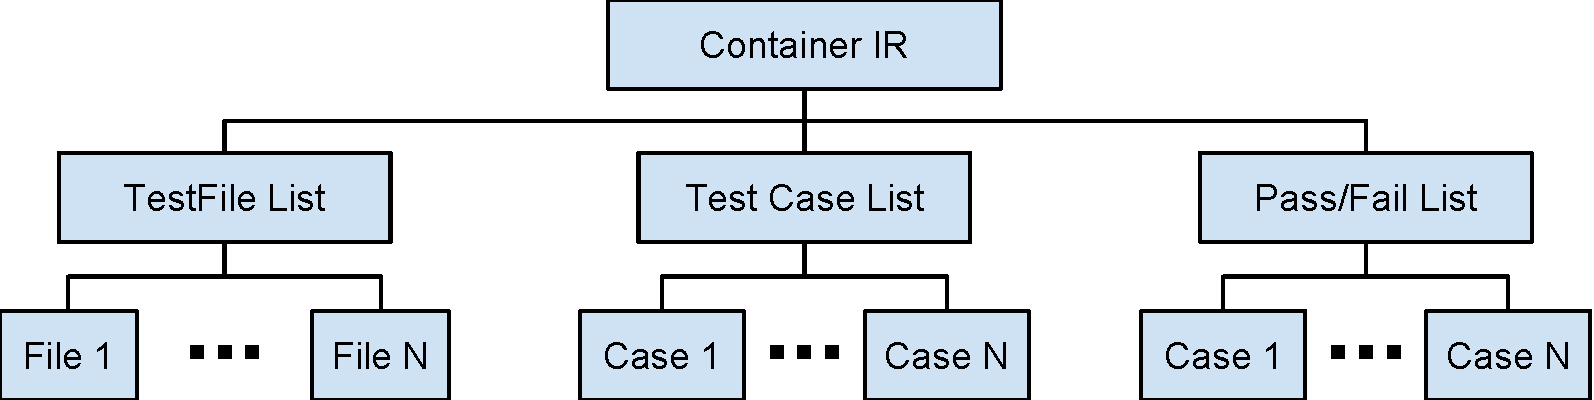
\includegraphics[width=0.8\linewidth]{img/ContainerIR.pdf}
\caption{Diagram of data structure for IR.}
\label{fig:ir}
\end{figure}

\begin{figure}[tb]
\centering
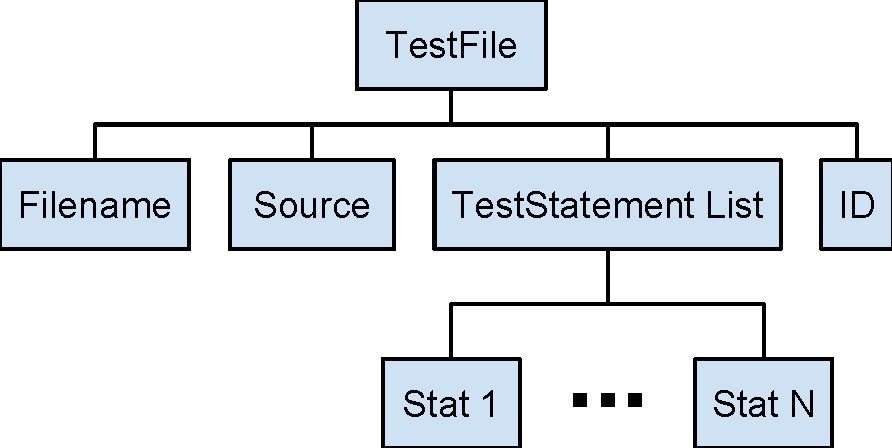
\includegraphics[height=30mm]{img/TestFile.pdf}
\hspace{0.1\linewidth}
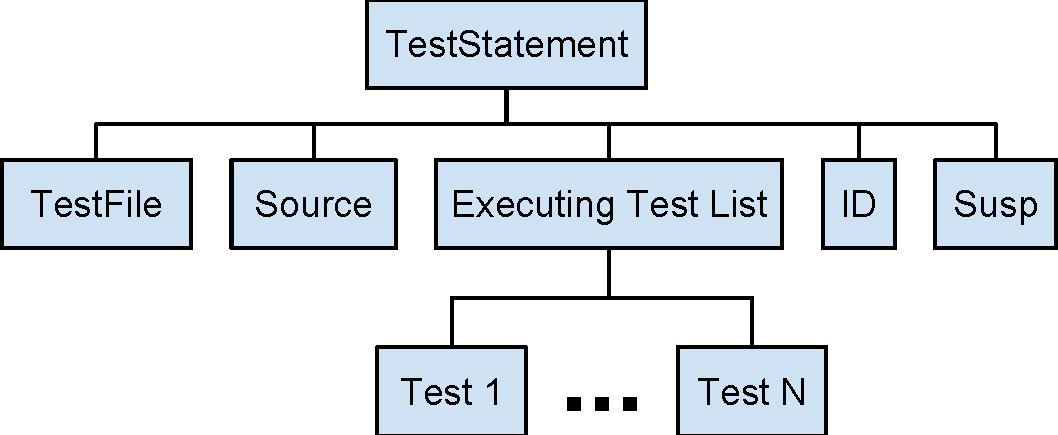
\includegraphics[height=30mm]{img/TestStatement.pdf}
\caption{Diagram of data structures used within the IR to store files (left) and 
statements (right)}
\label{fig:ir2}
\end{figure}

Each \texttt{TestFile} object contains the name and source code of the file as a \texttt{String}, the internal identification numberfor the file as an \texttt{int}, and a list of \texttt{TestStatement}s.  
A \texttt{TestStatement} includes an ID and source code for the statement, each stored as \texttt{String}s.  In addition, the \texttt{TestStatement} object stores a \texttt{TestFile} 
parent object and the suspiciousness value associated with the statement.  Finally, the statement 
includes a \texttt{boolean} list, where each element corresponds to a test case.  These boolean 
values indicate whether the respective test case executed this statment.  A \texttt{TestStatement} 
can be uniquely identified by the combination of its source file and ID.

CodeCover coverage containers include all required
information, divided into three sections.  First, the container lists all source
files included in coverage analysis, including the entirety of their source code,
the name of the file, and a unique internal identification value.  Following the source files
is a hierarchical list of all statements within those files.  These statements are defined by 
by their category, source file, and character offset within the source file.  For this
project, we only consider basic statements (in Java, this essentially refers to executable
statements terminated with semicolons).  

The final section of a CodeCover container is the per-test coverage data itself.  This is
represented by a series of test cases, each of which contains a child for every file
executed by that test. Under each file is a list of specific statements executed by that
test inside that file.  These statements are identified by their alphanumeric identifier.

Our system processes these sections in the order they appear above.  Using the DOM produced
from parsing, we can easily traverse the relevant segments of the container.  Traversal of
the DOM tree consists of repeated iterations of sub-levels of the XML hierarchy, in order
to locate a node with a specific name.  Throughout this process, we make no assumptions about
the sequence in which nodes appear.  Rather than assume that, for example, a given node is
always the first child, we always use a loop structure to make certain we identify the correct
node.

In order to identify all source files defined by the
XML container, we first locate the \texttt{SrcFileList} node.  We then iterate through its
children to locate all \texttt{SrcFile} nodes.  For each \texttt{SrcFile} node found, we 
extract the attributes of that node and add a \texttt{TestFile} to the \texttt{ContainerIR}
file list.  

Once we have located the source files, we must next identify the statements.  To do so, we first
locate the hierarchical statement definition root.  Beginning with that root node, we recursively
traverse the entire sub-tree.  For each \texttt{BasicStmnt} node, we add a new statement to the 
correct \texttt{TestFile}.  In order to do so, we must first identify the \texttt{LocList} child
node, followed by its \texttt{Loc} child node.  The attributes of the \texttt{Loc} node include
the source code character offset for the basic statement in question.  Between the attributes of
the \texttt{BasicStmnt} node and those of the \texttt{Loc} node, we extract the information
necessary to create a new \texttt{TestStatement} object.  Once this recursive traversal of the
statement hierarchy is complete, the \texttt{TestFile}s in the \texttt{ContainerIR} will contain
all basic statements.

Since we now have a complete list of basic statements, we can process the coverage data section
of the container to identify test cases and their coverage.  To begin, we first iteratively 
locate the \texttt{TestSession} node, whose children include a \texttt{TestCase} node for
each test case in the test suite.  We add the name of each test case to the \texttt{ContainerIR}
test case list, then process the children of the node to find coverage data.  Each test case
node contains a hierarchy of \texttt{CovList}, \texttt{CovPrefix}, and \texttt{Cov} nodes.  We 
locate all \texttt{CovPrefix} nodes, which each correspond to a single file, then retrieve the
\texttt{TestFile} corresponding to this node from the list of test files within the \texttt{ContainerIR}.
Finally, we iterate through all \texttt{Cov} children of the \texttt{CovPrefix} to find all 
basic statements covered by a given test case within a given file.  For each statement identified,
we mark the corresponding \texttt{TestStatement} as covered.

In addition to coverage data, a \texttt{TestCase} node also contains a \texttt{Comment} attribute.
This content of this attribute is comprised of the entire text output produced when the test case
was executed.  When the test case passes, this attribute is empty; however, when a failure occurs,
the description of the failure is stored in this node.  As a result, we can observe this attribute
to determine the pass/fail status of a given test.  We ascertain this data by checking the
\texttt{Comment} attribute for the starting string \texttt{"Failure"}.  Since this word always
heads the description of a failure, the \texttt{Comment} of a failed test will always begin with
the same text.  This pass/fail value is recorded in the boolean list stored in the 
\texttt{ContainerIR}, where true indicates a passed test and false indicates a failed one.  

\section{Simplified Representation} \label{sec:sir}

The intermediate representation discussed in section \ref{sec:ir} is appropriate as a preliminary
data structure.  However, it is not conducive to suspiciousness analysis.  All of the risk evaluation
functions considered in this project require four pieces of information for each statement that
must be evaluated: $ae_f, ae_p, an_f, \text{ and } an_p$ \cite{theory}.  These variables represent the number
of test cases that meet certain requirements for a given statement.  Variables $ae_f$ and $ae_p$
denote the number of test cases that executed the given statement and failed or passed
respectively. Similarly, $an_f$ and $an_p$ refer to the number of test cases that did not execute
the statement and passed or failed, respectively.  These four values become the input to each of
the suspiciousness functions.  Therefore, the simplified representation that best suits our needs
is one that stores these values for each statement, with no extraneous information.

Before converting the intermediate representation to the simplified form described above, we must
first address the issue of pass/fail status for test cases.  We resolve this problem by 
programmatically executing the JUnit test suite, with its class name provided at run time, that 
tests the system evaluated by CodeCover.  We achieve this by first using Java Reflection to 
acquire the \texttt{Class} object associated with the class name provided.  This \texttt{Class} then
becomes the input to \texttt{JUnitCore.run()}.  The \texttt{JUnitCore} class executes the
specified \texttt{Class} object, parsing the suite to locate all tests.  The \texttt{run()} 
method executes the test class, returning a \texttt{Result} object.

A \texttt{Result} object provides a list of \texttt{Failure} objects, which each includes the
fully qualified name of the test case that generated the error.  By extracting only the method
name portion of this full name, we can identify which test methods resulted in failures.  Since
CodeCover also by default uses test method names to label test cases, we can compare these values
directly to determine which of the test cases in the IR failed.  This provides the final necessary 
component for suspiciousness analysis.

In order to convert the IR to the described simple representation, the first step is build
a list of \texttt{TestInfo} objects, which represent individual test cases.  Each \texttt{TestInfo}
object includes a pass/fail boolean value, as well as a boolean list that describes, for each
statement under test, whether that statement was executed by this test.  We extract this information 
from the IR by iterating through the list of test case names.  For each test case, we check the
execution status of that test case for each statement, storing this information in a list (where
each element corresponds to a single statement, and true indicates the statement was executed by this
test).  Next, we compare the name of the test case in question to the list of failures provided
by the \texttt{Result} object discussed previously.  If the test case appears in the list of failures,
we mark the test as failing.

Iterating through the \texttt{TestInfo} list, we can determine the $ae_f, ae_p, an_f, \text{ and } an_p$
of each statement.  For each test case, we check whether the test passed then determine which statements
it executed by iterating through the boolean list stored in the \texttt{TestInfo} object.  For each
statement, we increment the appropriate variable depending on its pass/fail and execution status.  The
result is a list, for each of the four variables, in which each element corresponds to its value for
the corresponding statement.  After completing this process, we have a \texttt{CoverageReport} object
with all of the information necessary for risk evaluation.

\section{Risk Evaluation} \label{sec:re}

There are many different risk evaluation functions, but they are structurally similar.  We internally
represent risk evaluation functions using our \texttt{REFunction} interface.  This interface provides
abstract methods for returning the name of the function and for evaluating the function on provided
$ae_f, ae_p, an_f, \text{ and } an_p$.  Figure \ref{fig:re} provides an example implementation of
the REFunction interface.  For each function included, we create an implementation of
\texttt{REFunction}.  A complete list of \texttt{REFunctions} is stored in a static array of the
same name in \texttt{CoverageReport} for ease of iteratively performing all evaluation functions.  

\begin{figure}[tb]
\centering
\begin{lstlisting}
public class Jaccard implements REFunction {
	public double analyze( int aef, int aep, int anf, int anp ) {
		return ( (double) aef / (aef + anf + aep ) );
	}

	public String toString() {
		return "Jaccard";
	}
}
\end{lstlisting}

\caption{Implementation of REFunction interface for Jaccard function.}
\label{fig:re}
\end{figure}

When performing risk evaluation, we iterate through the specified functions.  For each of these
functions, we store the results of analysis in a \texttt{ResultsList} data structure.  This
structure allows for ease of sorting analyzed statements by suspiciousness rating.  In addition, the
suspiciousness values of the \texttt{ResultsList} are normalized to a zero-to-one scale according to

\[ L_i = \frac{ L_i - L_{min} }{ L_{max} - L_{min} }. \]

In this equation, $L_i$ refers to the $i^{th}$ element of the \texttt{ResultsList}, and $L_{max}, L_{min}$ refer to the maximum and minimum values in the list, respectively.  Though normalizing the results does
not change the ordering of the statements, it does make the actual suspiciousness values easier to compare
across multiple different functions.  The final result of analysis is a list of statements, ordered from
most suspicious to least suspicious, with values ranging from zero (not suspicious) to one (very 
suspicious).

\section{Overview} \label{sec:over}

When executing the system, the main class, \texttt{Test.java}, must be invoked with three additional
parameters.  The first of these is the fully qualified name of the JUnit test class (e.g. \texttt{edu.allegheny.listswap.ListSwapGeneratorTest}), which will be programmatically executed to
obtain pass/fail information.  This test class \emph{must} be in the classpath, or the system will
not be able to execute the tests.  The second parameter is the fully qualified file name for the 
CodeCover container to be analyzed.  The final parameter is the name for the output file---the 
output path is fixed to the (to be created) results directory within the present working directory.

Execution begins with parsing the XML container.  When the document has been stored as a DOM, it is
passed forward to the \texttt{ContainerIR} constructor, which processes the document into an IR as
described previously.  The IR is then passed to the \texttt{CoverageReport} class, where the 
test class is executed and coverage information is collated into the simple representation.
Suspiciousness evaluation is then completed using all risk evaluation functions specified.

After performing suspiciousness evaluation, the results are written to an output file in CSV (comma
separated value) format.  The attributes \textit{Function, Statement ID, Filename, Suspiciousness, Rank,
Statement Count,}
and \textit{Case Application} serve to uniquely identify a statement while providing information on risk evaluation.  
This format conforms to \textit{tidy data}  \cite{tidy}, a ``standard way of mapping the meaning of a 
dataset to its structure'', in that each variable forms a column and each observation forms a row.  
This organizational structure allows for reliably simple evaluation of data using statistical 
analysis tools.  Though tidy data contains extensive redundancy, that redundancy simplifies
the data analysis and visualization process.

%\section{Test Environment}
%Algorithm \ref{widgmin} (from \cite{Fiori:2013}) shows a high-level description of an
%algorithm. There are many options for the display of
%pseudocode; this uses the {\tt algorithm2e} package \cite{Fiori:2013}, 
%but there are a number of others available at the Comprehensive \TeX\ Archive
%Network (\url{ctan.org}). Using any of these
%other packages might require the additon of one or more
%``\verb$\usepackage{...}$'' commands in the main {\tt AllegThesis.tex} file.
%
%%   *******************************************************************
%%   * SEE CHAPTER ch_01overview.tex FOR INFORMATION ON CONTROLLING    *
%%   * PLACEMENT OF FIGURES.                                           *
%%   *                                                                 *
%%   * THERE ARE MANY DIFFERENT ALGORITHM ENVIRONMENTS. HERE, WE USE   *
%%   * THE "algorithm2e" PACKAGE, BUT YOU SHOULD LOOK TO SEE IF        *
%%   * OTHER PACKAGES BETTER MEET YOUR NEEDS. REGARDLESS OF WHICH      *
%%   * PACKAGE YOU USE, EXPECT TO SPEND TIME READING THE USER MANUAL   *
%%   * AS THERE ARE USUALLY A LARGE NUMBER OF PARAMETERS THAT CAN      *
%%   * SIGNIFICANTLY AFFECT THE FINAL APPEARANCE OF THE ALGORITHM.     *
%%   *******************************************************************
%
%\begin{algorithm}[htbp]
% %\SetLine % For v3.9
% \SetAlgoLined % For previous releases [?]
% \KwData{this text}
% \KwResult{how to write algorithm with \LaTeX2e }
% initialization\;
% \While{not at end of this document}{
%  read current\;
%  \eIf{understand}{
%   go to next section\;
%   current section becomes this one\;
%   }{
%   go back to the beginning of current section\;
%  }
% }
% \caption{How to write algorithms (from \cite{Fiori:2013})}
%\label{widgmin}
%\end{algorithm}
%
%\section{Experiments}
%
%Figure \ref{javaprog} shows a Java program. There are many, many options for
%providing program listings; only a few of the basic ones are shown
%in the figure. Some thought must be given to making code suitable
%for display in a paper. In particular long lines, tabbed indents, and
%several other practices should be avoided. Figure \ref{javaprog} makes
%use of the {\tt listings} style file \cite{Heinz:2013}.
%
%%   *******************************************************************
%%   * SEE CHAPTER ch_01overview.tex FOR INFORMATION ON CONTROLLING    *
%%   * PLACEMENT OF FIGURES.                                           *
%%   *                                                                 *
%%   * SEE THE MAIN FILE "AllegThesis.tex" FOR THE "\lstset" COMMAND   *
%%   * THAT DEFINES HOW PROGRAM LISTINGS WILL LOOK.                    *
%%   *                                                                 *
%%   * AS WITH EVERYTHING IN LATEX, LOOK AT THE USER MANUAL, SEARCH    *
%%   * FOR EXAMPLES ONLINE, CUSTOMIZE TO GET A PLEASING LOOK.          *
%%   *******************************************************************
%
%
%\begin{figure}[htbp]
%\centering
%\lstinputlisting{SampleProgUncommented.java}
%\caption{{\tt SampleProg}: A very simple program}
%\label{javaprog}
%\end{figure}
%
%\section{Threats to Validity}
%
